\documentclass[letterpaper,10pt]{article}
\usepackage[utf8]{inputenc}
\usepackage{fullpage}
\usepackage[english]{babel}
\usepackage{amsmath}
\usepackage{caption}
\usepackage{subcaption}
\usepackage{graphicx}
\usepackage{amssymb}

\renewcommand{\arraystretch}{1.4}
\setlength{\parindent}{0cm}

\begin{document}

\noindent
\begin{flushright}
    \large\textbf{Miguel Alcón Doganoc} \\
    Combinatorial Problem Solving \\
    May 7, 2019
\end{flushright}

\newcommand{\code}[1]{\texttt{#1}}

\noindent
{\huge{\textbf{Logic Synthesis}}}

\section{Description of the problem}
In this project, our goal is to solve the \textit{NOR Logic Synthesis Problem}
(NLSP): given a specification of a Boolean function $f(x_1,...,x_n)$ in the form of a truth table, find a NOR-circuit satisfying the specification that minimizes depth (and, in case of a tie in depth, with minimum size). An instance of NLSP consists in:
\begin{itemize}
    \item $\mathbf{n} := $ ``Number of input signals''
    \item $\mathbf{y_t} := $ ``Desired output signal, described by row $t$ in the truth table'', where $t \in \{0,1,...,2^n-1\}$  
\end{itemize}

\section{Decision variables}
Given the number of input signals $n$, the depth $d$, and the truth table of the logical circuit, I defined the following variables:
\begin{itemize}
    \item $\mathbf{Z_{i,j}}:=$ ``The node ($i$,$j$) contains a constant zero'', where
    \begin{itemize}
        \item $0 \leq i \leq d$
        \item $0 \leq j < 2^i$
    \end{itemize}
    \item $\mathbf{N_{i,j}}:=$ ``The node ($i$,$j$) contains a NOR gate'', where
    \begin{itemize}
        \item $0 \leq i \leq d$
        \item $0 \leq j < 2^i$
    \end{itemize}
    \item $\mathbf{I_{i,j,k}}:=$ ``The node ($i$,$j$) contains the input $k$'', where
    \begin{itemize}
        \item $0 \leq i \leq d$
        \item $0 \leq j < 2^i$
        \item $1 \leq k \leq n$
    \end{itemize}
    \item $\mathbf{B_{i,j}^{(t)}}:=$ ``Boolean value of the node ($i,j$) for the row $t$ of the truth table'', where
    \begin{itemize}
        \item $0 \leq i \leq d$
        \item $0 \leq j < 2^i$
        \item $0 \leq t < 2^n$
    \end{itemize}
\end{itemize}

For example, for a NOR-circuit that implements the functionality of an AND gate (see figure \ref{fig:original}), with $n = d = 2$, one possible solution for the variables $c_{i,j}$ and $B_{i,j}^{(0)}$ is shown in figures \ref{subfig:ci} and \ref{subfig:bit}, respectively.
\begin{figure}[hbtp]
    \centering
    \begin{subfigure}[b]{0.45\textwidth}
        \raisebox{18mm}{\begin{tabular}{c c | c | c}
            $x_1$ & $x_2$ & $y$ & $t$\\ \hline
            0 & 0 & 0 & 0 \\
            0 & 1 & 0 & 1 \\
            1 & 0 & 0 & 2 \\
            1 & 1 & 1 & 3 \\
        \end{tabular}}
    \end{subfigure}\hspace{-0.2\textwidth}
    \begin{subfigure}[b]{0.45\textwidth}
        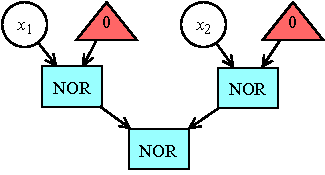
\includegraphics[width=\textwidth]{circuit.pdf}
    \end{subfigure}
    \caption{Truth table of $y$ = AND($x_1,x_2$) and NOR-circuit implementing it.}
    \label{fig:original}
\end{figure}

\begin{figure}[hbtp]
    \centering
    \begin{subfigure}[b]{0.30\textwidth}
        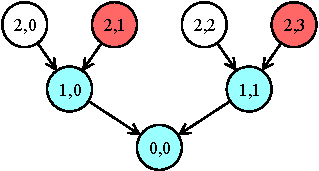
\includegraphics[width=\textwidth]{i.pdf}
        \caption{$i,j$}
        \label{subfig:i}
    \end{subfigure}
    \hspace{0.01\textwidth}
    \begin{subfigure}[b]{0.30\textwidth}
        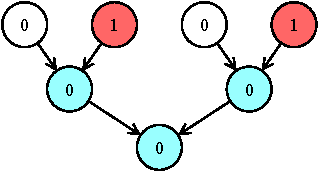
\includegraphics[width=\textwidth]{Z.pdf}
        \caption{$Z_{i,j}$}
        \label{subfig:ci}
    \end{subfigure}
    \hspace{0.01\textwidth}
    \begin{subfigure}[b]{0.30\textwidth}
        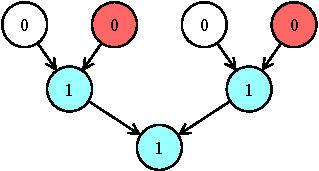
\includegraphics[width=\textwidth]{N.pdf}
        \caption{$N_{i,j}$}
        \label{subfig:ci}
    \end{subfigure}
    \begin{subfigure}[b]{0.30\textwidth}
        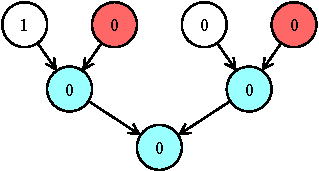
\includegraphics[width=\textwidth]{I1.pdf}
        \caption{$I_{i,j,1}$}
        \label{subfig:ci}
    \end{subfigure}
    \hspace{0.01\textwidth}
    \begin{subfigure}[b]{0.30\textwidth}
        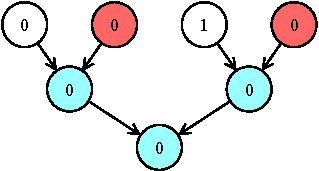
\includegraphics[width=\textwidth]{I2.pdf}
        \caption{$I_{i,j,2}$}
        \label{subfig:ci}
    \end{subfigure}
    \hspace{0.01\textwidth}
    \begin{subfigure}[b]{0.30\textwidth}
        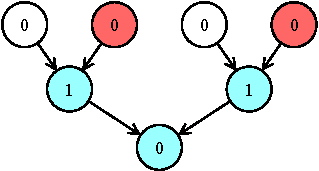
\includegraphics[width=\textwidth]{bit.pdf}
        \caption{$B_{i,j}^{(0)}$}
        \label{subfig:bit}
    \end{subfigure}
    \caption{Visual representation of ($i,j$) and the variables.}
    \label{fig:variables}
\end{figure}


\section{Constraints}
In order to simplify the definition of the constraints, I define three functions. Given the variable $v_{i,j}$, with $v_{i,j} \in \{Z_{i,j}; N_{i,j}; I_{i,j,k}; B_{i,j}^{(t)}\}$,
\begin{itemize}
    \item \textbf{left($v_{i,j}$)} := ``Variable corresponding to the one on the left of $v_{i,j}$'' $ = v_{i+1,2\times j}$.
    \item \textbf{right($v_{i,j}$)} := ``Variable corresponding to the one on the right of $v_{i,j}$'' $ = v_{i+1,2\times j+1}$.
    \item \textbf{bit($k,t$)} := ``Boolean value of $x_k$ in the $t$ row of the truth table'' = ``Value of the position $k$ of the binary representation of $t$ (i.e. $t_k \in \{t_1 t_2 ... t_n$\})''.
\end{itemize}

So, the constraints are the following:
\begin{itemize}
    \item The output of the circuit is equal to the desired value for each row $t$ of the truth table.
    \begin{align*}
        b_{0,0}^{(t)} = y_t \\
        \forall t < 2^n
    \end{align*}
    \item NOR gates are not allowed on the leaves of the circuit.
    \begin{align*}
        c_{d,j} \geq 0 \\
        \forall j < 2^d 
    \end{align*}
    \item Force children (if any) of each node to be 0 if the node is not a NOR gate.
    \begin{align*}
        c_{i,j} \geq 0 \Rightarrow (\mathbf{left}(c_{i,j}) = 0 \land \mathbf{right}(c_{i,j}) = 0) \\
        \forall i < d\text{ }\forall j < 2^i
    \end{align*}
    \item Force the left child of NOR gates to be greater or equal than the right one (non-symmetry of NOR gates).
    \begin{align*}
        c_{i,j} = -1 \Rightarrow (\mathbf{left}(c_{i,j}) \geq \mathbf{right}(c_{i,j})) \\
        \forall i < d\text{ }\forall j < 2^i
    \end{align*}
    \item Force the left child of NOR gates to be greater than the right one if one of them is an input signal (non-symmetry of NOR gates).
    \begin{align*}
        (c_{i,j} = -1 \land (\mathbf{left}(c_{i,j}) > 0 \lor \mathbf{right}(c_{i,j}) > 0)) \Rightarrow (\mathbf{left}(c_{i,j}) > \mathbf{right}(c_{i,j})) \\
        \forall i < d\text{ }\forall j < 2^i
    \end{align*}
    \item Link each NOR gate with its corresponding value, which is the NOR operation between both children.
    \begin{align*}
        c_{i,j} = -1 \Rightarrow (B_{i,j}^{(t)} = \lnot (\mathbf{left}(B_{i,j}^{(t)}) \lor \mathbf{right}(B_{i,j}^{(t)}))) \\
        \forall t < 2^n\text{ }\forall i < d\text{ }\forall j < 2^i
    \end{align*}
    \item Link each constant 0 signal with `false'.
    \begin{align*}
        c_{i,j} = 0 \Rightarrow \lnot B_{i,j}^{(t)} \\
        \forall t < 2^n\text{ }\forall i \leq d\text{ }\forall j < 2^i
    \end{align*}
    \item Link each input signal that has value 1 in the truth table, with `true'.
    \begin{align*}
        c_{i,j} = k \Rightarrow B_{i,j}^{(t)} \\
        \forall 1 \leq k \leq n\text{ }\forall t  < 2^n\text{ }\forall i \leq d\text{ }\forall j < 2^i\text{ where \textbf{bit($k,t$)}} = 1
    \end{align*}
    \item Link each input signal that has value 0 in the truth table, with `false'.
    \begin{align*}
        c_{i,j} = k \Rightarrow \lnot B_{i,j}^{(t)} \\
        \forall 1 \leq k \leq n\text{ }\forall t < 2^n\text{ }\forall i \leq d\text{ }\forall j < 2^i\text{ where \textbf{bit($k,t$)} }= 0
    \end{align*}
\end{itemize}

\section{Relation between the documentation and the code}
\subsection{Variables}
\begin{itemize}
    \item \code{IntVarArray circuit = }$\{c_{0,0},c_{1,0},c_{1,1},...,c_{d,2^d-1}\}$.
    \item For each $t$, which in the code is \code{truth\_idx}, \code{BoolVarArray circuit\_bool = }$\{b_{0,0}^{(t)},b_{1,0}^{(t)},b_{1,1}^{(t)},...,b_{d,2^d-1}^{(t)}\}$.
\end{itemize}
\subsection{Functions}
\begin{itemize}
    \item \textbf{left{($i,j$)}} and \textbf{right($v_{i,j}$)} are not directly implemented as functions.
    \item Function \code{bool is\_bit\_up(bit\_pos, number)} = \textbf{bit($k,t$)}.
\end{itemize}
\subsection{Others}
\begin{itemize}
    \item Most of the constrains are defined within the recursive function \code{constraint\_creation(...)}, accessing to variables like a tree.
    \item The algorithm tries to solve the problem from \textit{depth} 0 to \code{MAX\_DEPTH}, which is equal to 5, and stops in the first \textit{depth} where it finds a solution. 
    \item I used 4 threads when solving the instances.
\end{itemize}

\end{document}